\section{Objetos, classes, mensagens, argumentos}

SuperCollider é uma linguagem de programação orientada a objetos, como Java ou C++. Está além do escopo deste tutorial explicar o que isso significa, então deixaremos você pesquisar isso na internet se tiver curiosidade. Aqui vamos apenas explicar alguns conceitos básicos que você precisa saber para entender melhor esta nova linguagem que você está aprendendo.

Tudo no SuperCollider é um \emph{objeto}. Mesmo simples números são objetos no SC. Diferentes objetos se comportam de diferentes maneiras e armazenam diferentes tipos de informação. Você pode solicitar uma informação ou ação de um objeto enviando uma \emph{mensagem} para ele. Quando você escreve algo como \texttt{2.squared}, a mensagem \texttt{squared} está sendo enviada para o objeto \texttt{2}, que a recebe (por isso vamos chamá-lo de "objeto recebedor", tradução do inglês "receiver object"). O ponto entre o objeto e a mensagem faz a conexão entre os dois. A propósito, mensagens também são chamadas \emph{métodos}.

Objetos são especificados hierarquicamente em \emph{classes}. O SuperCollider vem com uma imensa coleção de classes pré-definidas, cada uma com seu próprio conjunto de métodos. 

Eis uma analogia pra ajudar a entender isso. Imaginemos que há uma classe abstrata de objetos chamada \texttt{Animal}. A classe Animal define alguns métodos (mensagens) comuns a todos os animais. Métodos como \texttt{mover}, \texttt{comer}, \texttt{dormir} fariam o Animal realizar uma ação específica. Daí poderíamos imaginar duas subclasses de Animal: uma chamada \texttt{Doméstico} outra chamada \texttt{Selvagem}. Cada uma destas subclasses poderia ter ainda mais subclasses derivadas destas (como \texttt{Cachorro} e \texttt{Gato}, derivados de \texttt{Doméstico}). Subclasses herdam todos os métodos de suas classes-mãe e implementam novos métodos próprios para atributos especializados. Por exemplo, tanto o objeto Cachorro quanto Gato alegremente responderiam à mensagem \texttt{.comer}, herdada da classe Animal. \texttt{Cachorro.nome} e \texttt{Gato.nome} retornariam o nome do bicho: \texttt{nome} poderia ser um método comum a todos os objetos derivados da classe Doméstico. \texttt{Cachorro} tem um método \texttt{latir}, então você pode chamar \texttt{Cachorro.latir} e ele saberá o que fazer. \texttt{Gato.latir} retornaria uma mensagem de erro: \texttt{ERRO: Mensagem ‘latir’ não entendida.}

Em todos estes exemplos hipotéticos, as palavras começando com uma letra maiúscula são \emph{classes} que representam \emph{objetos}. As palavras e minúsculas depois do ponto são \emph{mensagens} (ou \emph{métodos}) que estão sendo enviadas para estes objetos. Mandar uma mensagem para um objeto sempre retorna algum tipo de informação. Finalmente, mensagens às vezes aceitam (ou mesmo exigem) \emph{argumentos}. Argumentos são os dados que vêm entre parênteses logo depois de uma mensagem. Em \texttt{Gato.comer("sardinhas", 2)}, a mensagem \texttt{comer} está sendo enviada para \texttt{Gato} com algumas informações bem específicas: o que comer e em que quantidade. Às vezes você verá argumentos declarados explicitamente dentro de parênteses (palavras-chave terminando com dois pontos). Isso é muitas vezes útil para quem lê o código lembrar rapidamente a que o argumento se refere. \texttt{Cachorro.latir(volume: 10)} é mais autoexplicativo que apenas \texttt{Cachorro.latir(10)}.

\begin{figure}[h]
\centerline{\framebox{
	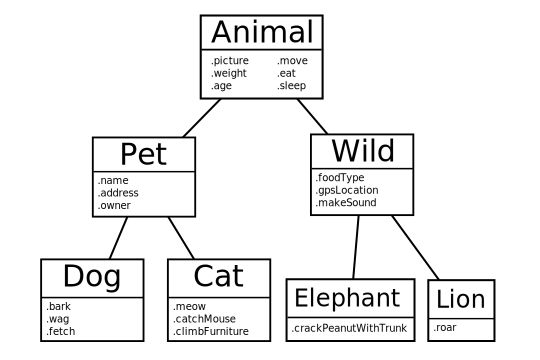
\includegraphics[scale=0.9]{fig-animal-class-chart.pdf}}}
\caption{Hierarquia de classes hipotética.}
\label{fig:animal-class-chart}
\end{figure}

OK---já basta desta explicação rapidinha sobre programação orientada a objetos. Vamos tentar alguns exemplos que você possa de fato rodar no SuperCollider. Rode uma linha após a outra e veja se você consegue identificar a mensagem, o objeto recebedor e o argumento (se houver). A estrutura básica é \texttt{Recebedor.mensagem(argumentos)}. Respostas ao final do livro.\endnote{Primeira linha: o Array \texttt{[1, 2, 3, "uau"]} é o objeto recebedor; \texttt{reverse} é a mensagem. Segunda linha: a String "alô" é o objeto recebedor; \texttt{dup} é a mensagem; \texttt{4} é o argumento para \texttt{dup}. Terceira linha: 3.1415 é o objeto recebedor; \texttt{round} é a mensagem; \texttt{0.1} é o argumento para \texttt{round}. Quarta linha: \texttt{100} é o objeto recebedor, \texttt{rand} é a mensagem. Última linha: \texttt{100.0} é o recebedor da mensagem \texttt{rand}, o resultado do qual é um número aleatório entre 0 e 100. Este número se torna o recebedor da mensagem \texttt{round} com o argumento \texttt{0.01}, assim o número aleatório é arredondado em duas casas decimais. Daí este resultado se torna o objeto recebedor da mensagem \texttt{dup} com o argumento \texttt{4}, que cria uma lista com quatro duplicatas daquele número.}

 
\begin{lstlisting}[style=SuperCollider-IDE, basicstyle=\scttfamily\footnotesize]
[1, 2, 3, "uau"].reverse;
"alô".dup(4); 
3.1415.round(0.1); // note que o primeiro ponto é a separação decimal de 3.1415 [N.T.: Atenção: o SC separa casas decimais com ponto! Vírgulas têm outros usos.]
100.rand; // rode esta linha diversas vezes;
// Encadear mensagens é divertido:
100.0.rand.round(0.01).dup(4);
\end{lstlisting}
